\chapter{{{Prototipe Protokol Komunikasi Memanfaatkan Sistem \emph{Chaos}}}} 
\label{appendix:protokol}

Figur \ref{fig:solution.protocol} merupakan prototipe protokol komunikasi memanfaatkan sistem \emph{chaos}. Pada awal komunikasi, akan dilakukan pertukaran kunci memanfaatkan algoritma \emph{Diffie-Hellman}. Selanjutnya, akan dikirimkan pesan hello oleh Alice dan Bob. Hal ini dilakukan untuk memverifikasi bahwa kedua pihak telah memiliki status kunci yang sama dalam melakukan enkripsi dan dekripsi. Apabila terjadi kegagalan pada tahap ini, koneksi harus diputus dan dibentuk koneksi yang baru.

\begin{figure}[!h]
  \centering
  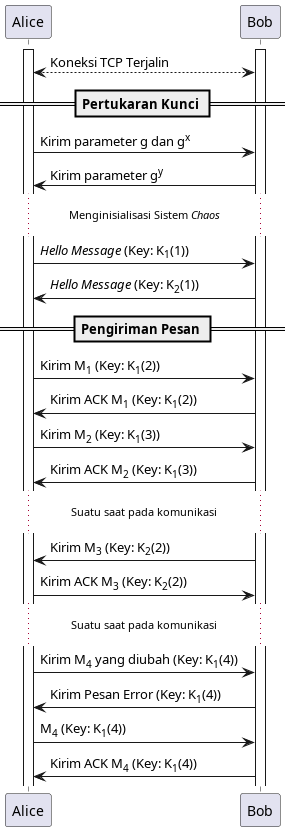
\includegraphics[width=200px]{chapters/res/chapter-3/img/protocol.png}
  \caption{Protokol Pengiriman Pesan} \label{fig:solution.protocol}
\end{figure}

Pada saat pengiriman data, Alice memanfaatkan sistem \emph{chaos} $K_1$, sedangkan Bob memanfaatkan sistem \emph{chaos} $K_2$. Pada saat mengirim data, Alice akan melakukan enkripsi pesan pada blok $n$. Setelah melakukan enkripsi, Alice akan memperbaharui sistem chaosnya. Setelah memperbaharui, Alice akan mengirimkan pesan blok $n$. Alice akan menunggu hingga pesan ACK dari Bob diterima sebelum mengirimkan blok selanjutnya. Alice akan mengirimkan kembali pesan blok $n$ bila belum mendapatkan ACK dalam waktu tertentu atau menerima pesan error.

Bob akan menerima data dari Alice. Apabila pesan memiliki HMAC yang benar, bob akan melakukan dekripsi. Setelah dekripsi berhasil, Bob akan mengirimkan ACK menuju Alice. Sistem \emph{chaos} Bob diperbaharui pada saat bob mendapatkan pesan blok $n+1$ yang valid.
